\documentclass[tikz]{standalone}
\usepackage{tikz}
\begin{document}
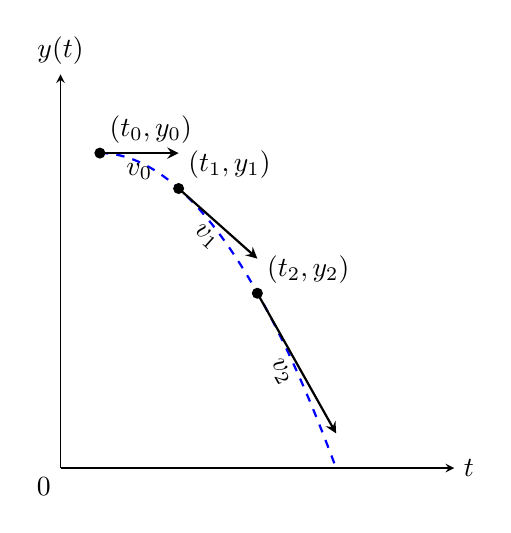
\begin{tikzpicture}[>=stealth]
    % Achsen
    \draw[->] (0,0) -- (5,0) node[right] {$t$};
    \draw[->] (0,0) -- (0,5) node[above] {$y(t)$};
    \node[below left] at (0,0) {$0$};

    % Flugbahn
    \draw[blue, thick, dashed] (0.5, 4) parabola (3.5, 0);
    
    % Startpunkt und Geschwindigkeit v0
    \fill (0.5,4) circle (2pt) node[above right] {$(t_0, y_0)$};
    \draw[->, thick] (0.5,4) -- (1.5, 4) node[midway, below, sloped] {$v_0$};

    % Punkt 1 und Geschwindigkeit v1
    % t = 1.5, y(1.5) = 3.55 (approx)
    % vy(1.5) = -0.89 (approx)
    \fill (1.5, 3.55) circle (2pt) node[above right] {$(t_1, y_1)$};
    \draw[->, thick] (1.5, 3.55) -- (2.5, 2.66) node[midway, below, sloped] {$v_1$};

    % Punkt 2 und Geschwindigkeit v2
    % t = 2.5, y(2.5) = 2.22 (approx)
    % vy(2.5) = -1.78 (approx)
    \fill (2.5, 2.22) circle (2pt) node[above right] {$(t_2, y_2)$};
    \draw[->, thick] (2.5, 2.22) -- (3.5, 0.44) node[midway, below, sloped] {$v_2$};
\end{tikzpicture}
\end{document}

